
%%%%%%%%%%%%%%%%%%%%%%%%%%%%%%%%%%%%%%%%%%%%%%%%%%%%%%%%%%%%%%%%%%%%%%%%%%%%%
\chapt[chap:developer]{Using GATE Developer}
\markboth{Using GATE Developer}{Using GATE Developer}
%%%%%%%%%%%%%%%%%%%%%%%%%%%%%%%%%%%%%%%%%%%%%%%%%%%%%%%%%%%%%%%%%%%%%%%%%%%%%
\nnormalsize
%%%% qqqqqqqqqqqqqqqqqqqqqqqqq %%%%
\ifprintedbook
\else
\begin{quote}
`The law of evolution is that the strongest survives!'

`Yes; and the strongest, in the existence of any social species, are
those who are most social. In human terms, most ethical.
\ldots There is no strength to be gained from
hurting one another. Only weakness.'

The Dispossessed [p.183], Ursula K. le Guin, 1974.
\end{quote}
\fi
%%%% qqqqqqqqqqqqqqqqqqqqqqqqq %%%%

%This \chapthing\ introduces GATE Developer, and describes how to complete
%common tasks. Probably the best way to learn how to use GATE Developer is to
%look at the \htlink{http://gate.ac.uk/demos/movies.html} {demonstrations and
%tutorials movies}. There are specific links to them in this \chapthing.

This \chapthing\ introduces GATE Developer, which is the GATE graphical
user interface. It is analogous to systems like Mathematica for mathematicians,
or Eclipse for Java programmers, providing a convenient graphical environment
for research and development of language processing software. As well as being a
powerful research tool in its own right, it is also very useful in conjunction
with GATE Embedded (the GATE API by which GATE functionality can be included in
your own applications); for example, GATE Developer can be used to create
applications that can then be embedded via the API. This \chapthing\ describes
how to complete common tasks using GATE Developer. It is intended to provide a good
entry point to GATE functionality, and so explanations are given assuming only
basic knowledge of GATE. However, probably the best way to learn how to use GATE
Developer is to use this \chapthing\ in conjunction with the
\htlink{http://gate.ac.uk/demos/movies.html} {demonstrations and tutorials
movies}. There are specific links to them throughout the \chapthing. There is
also a complete new set of video tutorials
\htlink{https://gate.ac.uk/demos/developer-videos/}{here}.

The basic business of GATE is annotating documents, and all the functionality 
we will introduce relates to that. Core concepts are;

\begin{itemize}
  \item the {\bf documents} to be annotated,
  \item {\bf corpora} comprising sets of documents, grouping documents for the
  purpose of running uniform processes across them,
  \item {\bf annotations} that are created on documents,
  \item {\bf annotation types} such as `Name' or `Date',
  \item {\bf annotation sets} comprising groups of annotations,
  \item {\bf processing resources} that manipulate and create annotations on
  documents, and
  \item {\bf applications}, comprising sequences of processing resources, that
  can be applied to a document or corpus.
\end{itemize}

What is considered to be the end result of the process varies depending on the
task, but for the purposes of this \chapthing, output takes the form of the
annotated document/corpus. Researchers might be more interested in figures
demonstrating how successfully their application compares to a `gold standard'
annotation set; \Chapthing~\ref{chap:eval} in Part \ref{part:advanced-gate} will
cover ways of comparing annotation sets to each other and obtaining measures such
as F1. Implementers might be more interested in using the annotations
programmatically; \Chapthing~\ref{chap:api}, also in Part
\ref{part:advanced-gate}, talks about working with annotations from GATE
Embedded. For the purposes of this chapter, however, we will focus only on
creating the annotated documents themselves, and creating GATE applications for
future use.

GATE includes a complete information extraction system that you are free to
use, called ANNIE (a Nearly-New Information Extraction System). Many users
find this is a good starting point for their own application, and so we will
cover it in this \chapthing. \Chapthing~\ref{chap:annie} talks in a lot more
detail about the inner workings of ANNIE, but we aim to get you started using
ANNIE from inside of GATE Developer in this chapter.

We start the \chapthing\ with an exploration of the GATE Developer GUI, in
Section \ref{sec:developer:gui}. We describe how to create documents
(Section~\ref{sec:developer:documents}) and corpora
(Section~\ref{sec:developer:loadlr}). We talk about viewing and manually
creating annotations (Section~\ref{sec:developer:annotations}).

We then talk about loading the plugins that contain the processing resources you
will use to construct your application, in Section~\ref{sec:developer:plugins}.
We then talk about instantiating processing resources
(Section~\ref{sec:developer:loadpr}). Section~\ref{sec:developer:apps} covers
applications, including using ANNIE (Section \ref{sec:developer:annie}). Saving
applications and language resources (documents and corpora) is covered in Section
\ref{sec:developer:saving}. We conclude with a few assorted topics that might be
useful to the GATE Developer user, in Section \ref{sec:developer:misc}.

%%%%%%%%%%%%%%%%%%%%%%%%%%%%%%%%%%%%%%%%%%%%%%%%%%%%%%%%%%%%%%%%%%%%%%%%%%%%%
%\sect[sec:developer:guistart]{Finding your Way in GATE Developer}
%%%%%%%%%%%%%%%%%%%%%%%%%%%%%%%%%%%%%%%%%%%%%%%%%%%%%%%%%%%%%%%%%%%%%%%%%%%%%
%
%This section describes what is where in GATE Developer. Section
%\ref{sec:developer:gui} covers the entire of the main window. Section
%\ref{sec:developer:documenteditor} focuses on the document editor pane, which
%appears when the main resource viewer is used to view a document.

%%%%%%%%%%%%%%%%%%%%%%%%%%%%%%%%%%%%%%%%%%%%%%%%%%%%%%%%%%%%%%%%%%%%%%%%%%%%%
\sect[sec:developer:gui]{The GATE Developer Main Window}
%%%%%%%%%%%%%%%%%%%%%%%%%%%%%%%%%%%%%%%%%%%%%%%%%%%%%%%%%%%%%%%%%%%%%%%%%%%%%

%
\begin{figure}[!htb]
\begin{center}
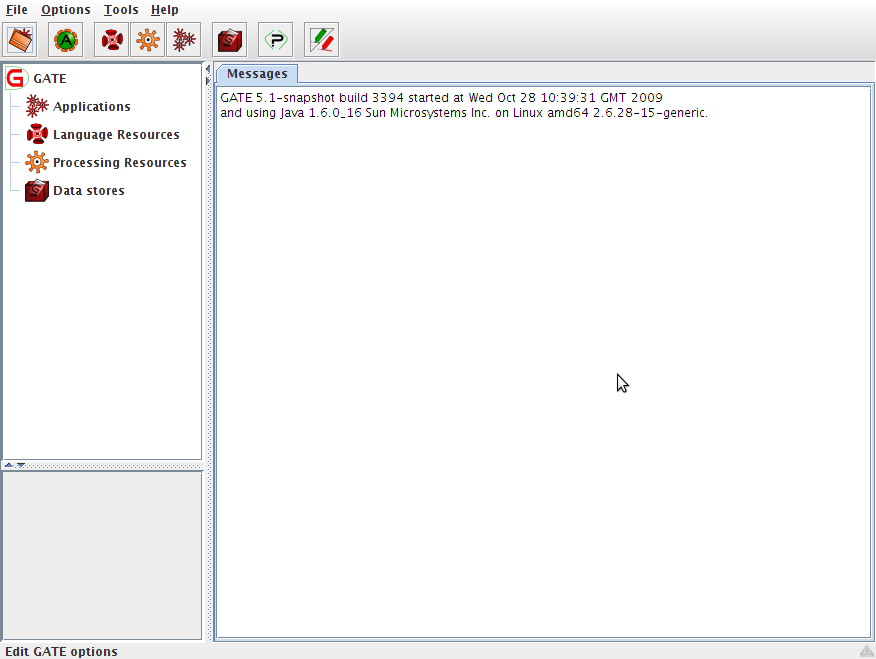
\includegraphics[width=14cm]{developer-clean-start.png}
\end{center}
\caption{Main Window of GATE Developer}
\label{fig:mainWindow1}
\end{figure}
%
Figure \ref{fig:mainWindow1} shows the main window of GATE Developer, as you
will see it when you first run it. There are five main areas:
%
\begin{enumerate}
\item\label{item:menubar}
at the top, the {\em menus bar} and {\em tools bar} with menus `File',
`Options', `Tools', `Help' and icons for the most frequently used actions;
\item\label{item:resourcetree}
on the left side, a tree starting from `GATE' and containing
`Applications', `Language Resources' etc. -- this is the {\em resources tree};
\item\label{item:smallresview}
in the bottom left corner, a rectangle, which is the {\em small resource
viewer};
\item\label{item:mainresview}
in the center, containing tabs with `Messages' or the name
of a resource from the resources tree, the {\em main resource viewer};
\item\label{item:messagebar}
at the bottom, the {\em messages bar}.
\end{enumerate}
%
The menu and the messages bar do the usual things. Longer messages are
displayed in the messages tab in the main resource viewer area.

The resource tree and resource viewer areas work together to allow the system
to display diverse resources in various ways. The many resources integrated
with GATE can have either a small view, a large view, or both.

At any time, the main viewer can also be used to display other
information, such as messages, by clicking on the appropriate tab at the top of 
the main window. If an error occurs in processing, the messages tab will flash 
red, and an additional popup error message may also occur.

In the options dialogue from the Options menu you can choose if you want to
link the selection in the resources tree and the selected main view.

%All the resources, applications and datastores currently loaded in the
%system appear in the resources tree; double clicking on a resource will load
%the viewer[s] for the resource in the resource view areas.

%You should next read the section \ref{sec:developer:load} to load creole resources.

%%%%%%%%%%%%%%%%%%%%%%%%%%%%%%%%%%%%%%%%%%%%%%%%%%%%%%%%%%%%%%%%%%%%%%%%%%%%%
\sect[sec:developer:documents]{Loading and Viewing Documents}
%%%%%%%%%%%%%%%%%%%%%%%%%%%%%%%%%%%%%%%%%%%%%%%%%%%%%%%%%%%%%%%%%%%%%%%%%%%%%

\begin{figure}[!htb]
\begin{center}
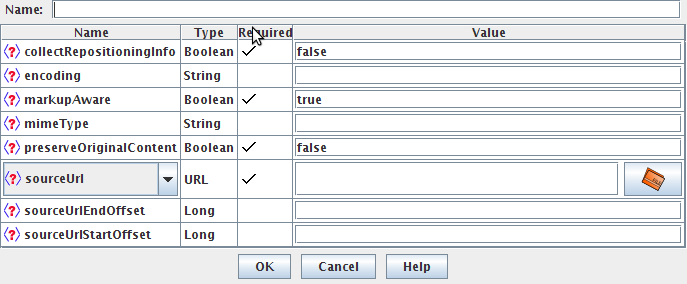
\includegraphics[width=14cm]{making-new-document.png}
\end{center}
\caption{Making a New Document}
\label{fig:making-new-document}
\end{figure}

If you right-click on `Language Resources' in the resources pane, select ``New'
then `GATE Document', the window `Parameters for the new GATE Document' will
appear as shown in figure~\ref{fig:making-new-document}. Here, you can specify
the GATE document to be created. Required parameters are indicated with a tick.
The name of the document will be created for you if you do not specify it. Enter
the URL of your document or use the file browser to indicate the file you wish to
use for your document source. For example, you might use `http://gate.ac.uk',
or browse to a text or XML file you have on disk. Click on `OK' and a GATE
document will be created from the source you specified.

See also the \htlink{http://gate.ac.uk/demos/movies.html\#loadDocs}
{movie for creating documents}.

%%%%%%%%%%%%%%%%%%%%%%%%%%%%%%%%%%%%%%%%%%%%%%%%%%%%%%%%%%%%%%%%%%%%%%%%%%%%%
%\subsect[sec:developer:documenteditor]{The Document Editor}
%%%%%%%%%%%%%%%%%%%%%%%%%%%%%%%%%%%%%%%%%%%%%%%%%%%%%%%%%%%%%%%%%%%%%%%%%%%%%

\begin{figure}[!htb]
\begin{center}
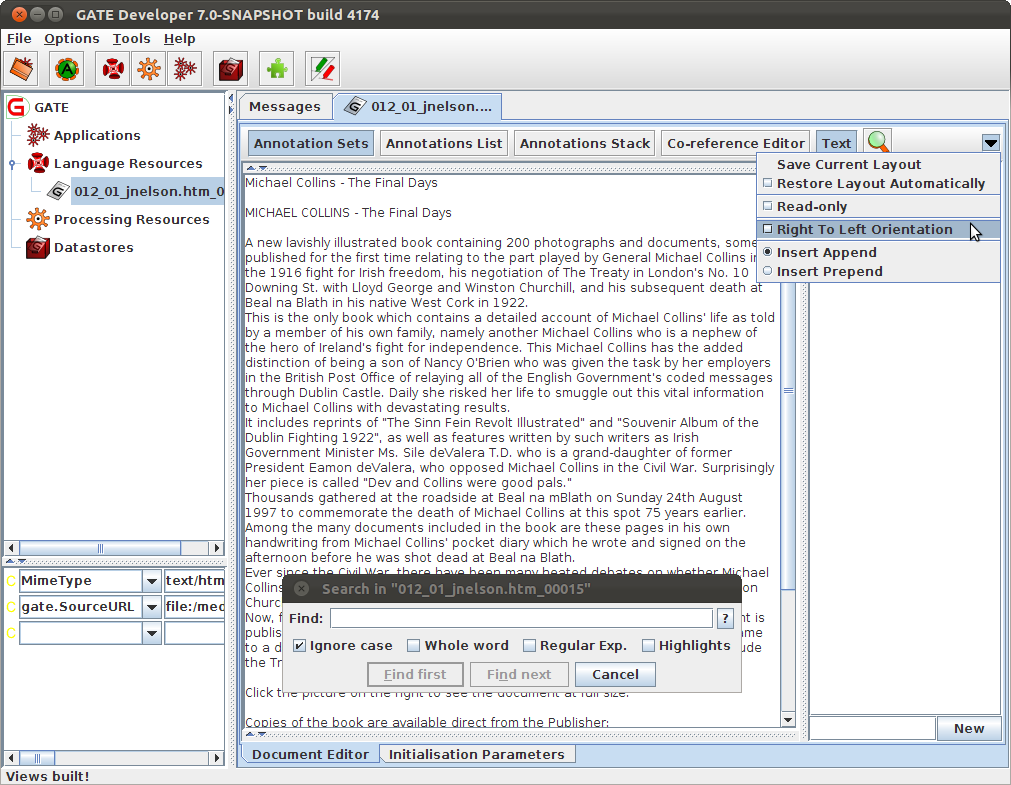
\includegraphics[width=14cm]{document-editor.png}
\end{center}
\caption{The Document Editor}
\label{fig:document-editor}
\end{figure}

The document editor is contained in the central tabbed pane in GATE Developer.
Double-click on your document in the resources pane to view the document editor.

The document editor consists of a top panel with buttons and icons that control
the display of different views and the search box. Initially, you will see just
the text of your document, as shown in figure~\ref{fig:document-editor}. Click on
`Annotation Sets' and `Annotations List' to view the annotation sets to the right
and the annotations list at the bottom.

You will see a view similar to
figure~\ref{fig:document-editor-with-annotations}. In place of the
annotations list, you can also choose to see the annotations stack. In place
of the annotation sets, you can also choose to view the co-reference
editor. More information about this functionality is given in
Section~\ref{sec:developer:annotations}.

Several options can be set from the small triangle icon at the top right
corner.

With `Save Current Layout' you store the way the different views are shown
and the annotation types highlighted in the document. Then if you set
`Restore Layout Automatically' you will get the same views and annotation
types each time you open a document. The layout is saved to the user
preferences file, gate.xml. It means that you can give this file to a new
user so s/he will have a preconfigured document editor.

Another setting make the document editor `Read-only'. If enabled, you won't
be able to edit the text but you will still be able to edit annotations. It
is useful to avoid to involuntarily modify the original text.

The option `Right To Left Orientation' is useful for changing orientation of
the text for the languages such as Arabic and Urdu.  Selecting this option 
changes orientation of the text of the currently visible document.

Finally you can choose between `Insert Append' and `Insert Prepend'.  That
setting is only relevant when you're inserting text at the very border of an
annotation.

If you place the cursor at the start of an annotation, in one case the newly
entered text will become part of the annotation, in the other case it will
stay outside. If you place the cursor at the end of an annotation, the
opposite will happen.

Let use this sentence: `This is an [annotation].' with the square brackets []
denoting the boundaries of the annotation. If we insert a `x' just before
the `a' or just after the `n' of `annotation', here's what we get:

Append
\begin{itemize}
\item This is an x[annotation].
\item This is an [annotationx].
\end{itemize}

Prepend
\begin{itemize}
\item This is an [xannotation].
\item This is an [annotation]x.
\end{itemize}

\begin{figure}[!htb]
\begin{center}
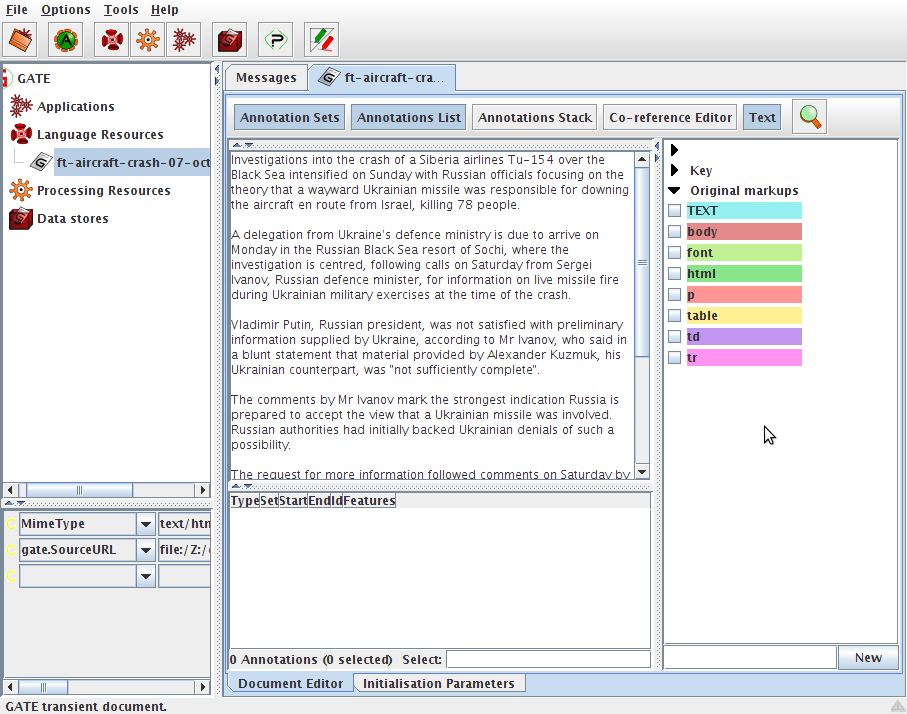
\includegraphics[width=14cm]{document-editor-with-annotations.png}
\end{center}
\caption{The Document Editor with Annotation Sets and Annotations List}
\label{fig:document-editor-with-annotations}
\end{figure}

Text in a loaded document can be edited in the document viewer. The usual
platform specific cut, copy and paste keyboard shortcuts should also work,
depending on your operating system (e.g. CTRL-C, CTRL-V for Windows). The
last icon, a magnifying glass, at the top of the document editor is for
searching in the document. To prevent the new annotation windows popping up
when a piece of text is selected, hold down the CTRL key. Alternatively, you 
can hide the annotation sets view by clicking on its button at the top of the
document view; this will also cause the highlighted portions of the text
to become un-highlighted.

See also Section \ref{sec:alignment:compunddoceditor} for the compound
document editor.

%%%%%%%%%%%%%%%%%%%%%%%%%%%%%%%%%%%%%%%%%%%%%%%%%%%%%%%%%%%%%%%%%%%%%%%%%%%%%
\sect[sec:developer:loadlr]{Creating and Viewing Corpora}
\label{sec:developer:corpuspopulate}
%%%%%%%%%%%%%%%%%%%%%%%%%%%%%%%%%%%%%%%%%%%%%%%%%%%%%%%%%%%%%%%%%%%%%%%%%%%%%

You can create a new corpus in a similar manner to creating a new document;
simply right-click on `Language Resources' in the resources pane, select `New'
then `GATE corpus'. A brief dialogue box will appear in which you can
optionally give a name for your corpus (if you leave this blank, a corpus name
will be created for you) and optionally add documents to the corpus from those
already loaded into GATE.

There are three ways of adding documents to a corpus:
\begin{enumerate}
  
\item When creating the corpus, clicking on the icon next to the
``documentsList'' input field brings up a popup window with a list of the 
documents already loaded into GATE Developer. This enables the user to add any
documents to the corpus.

\item Alternatively, the corpus can be loaded first, and documents added later
by double clicking on the corpus and using the + and - icons to add or remove
documents to the corpus. Note that the documents must have been loaded
into GATE Developer before they can be added to the corpus.

\item Once loaded, the corpus can be populated by right clicking on the corpus
and selecting `Populate'. With this method, documents do not have to have been
previously loaded into GATE Developer, as they will be loaded during the
population process. If you right-click on your corpus in the resources pane, you
will see that you have the option to `Populate' the corpus. If you select this
option, you will see a dialogue box in which you can specify a directory in which
GATE will search for documents. You can specify the extensions allowable; for
example, XML or TXT. This will restrict the corpus population to only those
documents with the extensions you wish to load. You can choose whether to recurse
through the directories contained within the target directory or restrict the
population to those documents contained in the top level directory. Click on `OK'
to populate your corpus. This option provides a quick way to create a GATE Corpus
from a directory of documents.

\end{enumerate}

Additionally, right-clicking on a loaded document in the tree and selecting
the `New corpus with this document' option creates a new transient corpus
named {\tt Corpus for {\em document name}} containing just this document.

See also the \htlink{http://gate.ac.uk/demos/movies.html\#corpora}
{movie for creating and populating corpora}.

%%%%%%%%%%%%%%%%%%%%%%%%%%%%%%%%%%%%%%%%%%%%%%%%%%%%%%%%%%%%%%%%%%%%%%%%%%%%%
%\subsect[sec:developer:corpuseditor]{The Corpus Editor}
%%%%%%%%%%%%%%%%%%%%%%%%%%%%%%%%%%%%%%%%%%%%%%%%%%%%%%%%%%%%%%%%%%%%%%%%%%%%%

\begin{figure}[htb]
\begin{center}
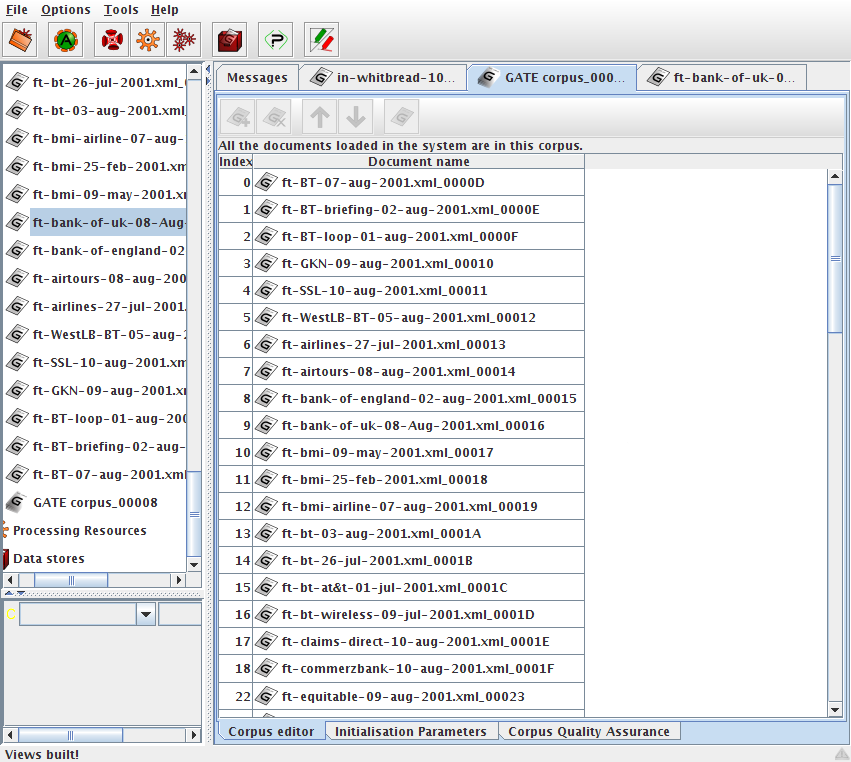
\includegraphics[width=14cm]{corpus-editor.png}
\end{center}
\caption{Corpus Editor}
\label{fig:corpuseditor}
\end{figure}

Double click on your corpus in the resources pane to see the corpus
editor, shown in figure~\ref{fig:corpuseditor}. You will see a list of the
documents contained within the corpus.

In the top left of the corpus editor, plus and minus buttons allow you to add
documents to the corpus from those already loaded into GATE and remove
documents from the corpus (note that removing a document from a corpus does not
remove it from GATE).

Up and down arrows at the top of the view allow you to reorder the documents in
the corpus. The rightmost button in the view opens the currently selected
document in a document editor.

At the bottom, you will see that tabs entitled `Initialisation Parameters' and
`Corpus Quality Assurance' are also available in addition to the corpus editor
tab you are currently looking at. Clicking on the `Initialisation Parameters' tab
allows you to view the initialisation parameters for the corpus. The `Corpus
Quality Assurance' tab allows you to calculate agreement measures between the
annotations in your corpus. Agreement measures are discussed in depth in
\Chapthing~\ref{chap:eval}. The use of corpus quality assurance is discussed in
Section~\ref{sec:eval:corpusqualityassurance}.

%%%%%%%%%%%%%%%%%%%%%%%%%%%%%%%%%%%%%%%%%%%%%%%%%%%%%%%%%%%%%%%%%%%%%%%%%%%%%
\sect[sec:developer:annotations]{Working with Annotations}
%%%%%%%%%%%%%%%%%%%%%%%%%%%%%%%%%%%%%%%%%%%%%%%%%%%%%%%%%%%%%%%%%%%%%%%%%%%%%

In this section, we will talk in more detail about viewing annotations, as well
as creating and editing them manually. As discussed in at the start of the
\chapthing, the main purpose of GATE is annotating documents. Whilst applications
can be used to annotate the documents entirely automatically, annotation can also
be done manually, e.g. by the user, or semi-automatically, by running an
application over the corpus and then correcting/adding new annotations manually.
Section~\ref{sec:developer:edit} focuses on manual annotation. In
Section~\ref{sec:developer:loadpr} we talk about running processing resources on
our documents. We begin by outlining the functionality around viewing
annotations, organised by the GUI area to which the functionality pertains.

%%%%%%%%%%%%%%%%%%%%%%%%%%%%%%%%%%%%%%%%%%%%%%%%%%%%%%%%%%%%%%%%%%%%%%%%%%%%%
\subsect[sec:developer:annotationsetsview]{The Annotation Sets View}
%%%%%%%%%%%%%%%%%%%%%%%%%%%%%%%%%%%%%%%%%%%%%%%%%%%%%%%%%%%%%%%%%%%%%%%%%%%%%

To view the annotation sets, click on the `Annotation Sets' button at the top of
the document editor, or use the F3 key (see Section~\ref{sec:developer:keyboard}
for more keyboard shortcuts). This will bring up the annotation sets viewer,
which displays the annotation sets available and their corresponding annotation
types.

The annotation sets view is displayed on the left part of the document
editor. It's a tree-like view with a root for each annotation set. The first
annotation set in the list is always a nameless set. This is the default
annotation set. You can see in
figure~\ref{fig:document-editor-with-annotations} that there is a drop-down
arrow with no name beside it. Other annotation sets on the document shown in
figure~\ref{fig:document-editor-with-annotations} are `Key' and `Original
markups'. Because the document is an XML document, the original XML markup is
retained in the form of an annotation set. This annotation set is expanded, and
you can see that there are annotations for `TEXT', `body', `font', `html', `p',
`table', `td' and `tr'.

To display all the annotations of one type, tick its checkbox or use the space
key. The text segments corresponding to these annotations will be highlighted in
the main text window. To delete an annotation type, use the delete key. To change
the color, use the enter key. There is a context menu for all these actions that
you can display by right-clicking on one annotation type, a selection or an
annotation set.

If you keep shift key pressed when you open the annotation sets view, GATE
Developer will try to select any annotations that were selected in the previous
document viewed (if any); otherwise no annotation will be selected.

Having selected an annotation type in the annotation sets view, hovering over an
annotation in the main resource viewer or right-clicking on it will bring up a
popup box containing a list of the annotations associated with it, from which
one can select an annotation to view in the annotation editor, or if there is
only one, the annotation editor for that annotation.
Figure~\ref{fig:annotations-editor} shows the annotation editor.

\begin{figure}[htb]
\begin{center}
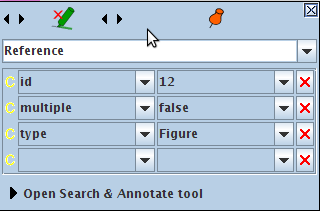
\includegraphics[scale=2]{annotations-editor.png}
\end{center}
\caption{The Annotation Editor}
\label{fig:annotations-editor}
\end{figure}

% To create a new annotation set use the text field at the bottom and the `New'
% button.

%%%%%%%%%%%%%%%%%%%%%%%%%%%%%%%%%%%%%%%%%%%%%%%%%%%%%%%%%%%%%%%%%%%%%%%%%%%%%
\subsect[sec:developer:annotationslistview]{The Annotations List View}
%%%%%%%%%%%%%%%%%%%%%%%%%%%%%%%%%%%%%%%%%%%%%%%%%%%%%%%%%%%%%%%%%%%%%%%%%%%%

To view the list of annotations and their features, click on the
`Annotations list' button at the top of the main window or use F4 key. The
annotation list view will appear below the main text. It will only contain
the annotations selected from the annotation sets view. These lists can be
sorted in ascending and descending order for any column, by clicking on the
corresponding column heading. Moreover you can hide a column by using the
context menu by right-clicking on the column headings. Selecting rows in the
table will blink the respective annotations in the document. Right-click on
a row or selection in this view to delete or edit an annotation. Delete key
is a shortcut to delete selected annotations.

%%%%%%%%%%%%%%%%%%%%%%%%%%%%%%%%%%%%%%%%%%%%%%%%%%%%%%%%%%%%%%%%%%%%%%%%%%%%
\subsect[sec:developer:annotationsstackview]{The Annotations Stack View}
%%%%%%%%%%%%%%%%%%%%%%%%%%%%%%%%%%%%%%%%%%%%%%%%%%%%%%%%%%%%%%%%%%%%%%%%%%%%

\begin{figure}[htb]
\begin{center}
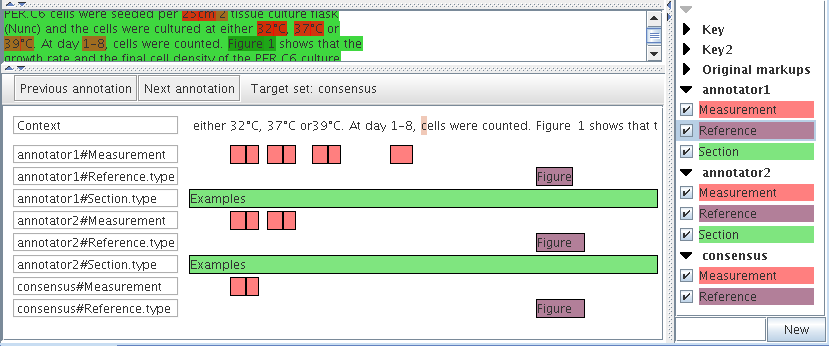
\includegraphics[width=14cm]{annotations-stack-view.png}
\end{center}
\caption{Annotations stack view centred on the document caret.}
\label{fig:annotationstackview}
\end{figure}

This view is similar to the ANNIC view described in
section~\ref{sec:annic:search-gui}. It displays annotations at the document
caret position with some context before and after. The annotations are
stacked from top to bottom, which gives a clear view when they are
overlapping.

As the view is centred on the document caret, you can use the conventional
key to move it and update the view: notably the keys left and right to skip
one letter; control + left/right to skip one word; up and down to go one
line up or down; and use the document scrollbar then click in the document
to move further.

There are two buttons at the top of the view that centre the view on the
closest previous/next annotation boundary among all displayed. This is
useful when you want to skip a region without annotation or when you want to
reach the beginning or end of a very long annotation.

The annotation types displayed correspond to those selected in the
annotation sets view. You can display feature values for an annotation
rectangle by hovering the mouse on it or select only one feature to display
by double-clicking on the annotation type in the first column.

Right-click on an annotation in the annotations stack view to edit
it. Control-Shift-click to delete it. Double-click to copy it to another
annotation set. Control-click on a feature value that contains an URL to
display it in your browser.

All of these mouse shortcuts make it easier to create a gold standard
annotation set.

%%%%%%%%%%%%%%%%%%%%%%%%%%%%%%%%%%%%%%%%%%%%%%%%%%%%%%%%%%%%%%%%%%%%%%%%%%%%%
\subsect[sec:developer:coreferenceeditor]{The Co-reference Editor}
%%%%%%%%%%%%%%%%%%%%%%%%%%%%%%%%%%%%%%%%%%%%%%%%%%%%%%%%%%%%%%%%%%%%%%%%%%%%%

\begin{figure}[htb]
\begin{center}
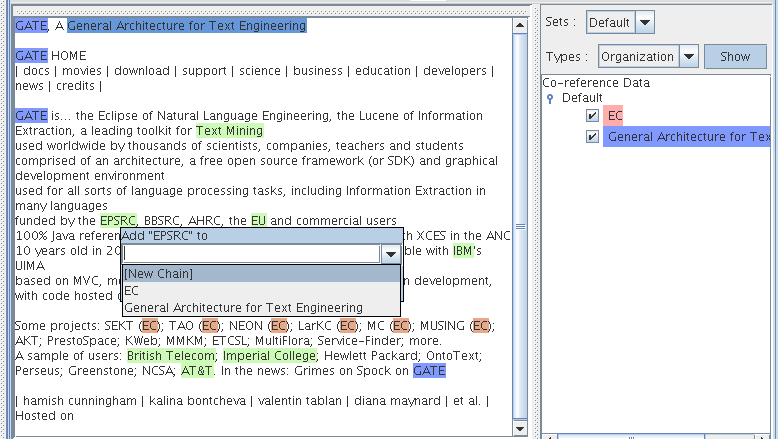
\includegraphics[scale=0.5]{co-reference-editor.png}
\end{center}
\caption{Co-reference editor inside a document editor. The popup window in
the document under the word `EPSRC' is used to add highlighted annotations
to a co-reference chain. Here the annotation type `Organization' of the
annotation set `Default' is highlighted and also the co-references `EC' and
`GATE'.}
\label{fig:coreferenceeditor}
\end{figure}

The co-reference editor allows co-reference chains (see Section 
\ref{sec:annie:pronom-coref}) to be displayed and edited in GATE Developer.
To display the co-reference editor, first open a document in GATE
Developer, and then click on the {\tt Co-reference Editor} button in
the document viewer.

The combo box at the top of the co-reference editor allows you to choose which 
annotation set to display co-references for. If an annotation set contains no
co-reference data, then the tree below the combo box will just show `Coreference
Data' and the name of the annotation set. However, when co-reference data does 
exist, a list of all the co-reference chains that are based on annotations in 
the currently selected set is displayed. The name of each co-reference chain in
this list is the same as the text of whichever element in the chain is the 
longest. It is possible to highlight all the 
member annotations of any chain by selecting it in the list.

When a co-reference chain is selected, if the mouse is placed over one of its
member annotations, then a pop-up box appears, giving the user the option
of deleting the item from the chain. If the only item in a chain is deleted, 
then the chain itself will cease to exist, and it will be removed from the list
of chains. If the name of the chain was derived from the item that was deleted,
then the chain will be given a new name based on the next longest item in the
chain.

A combo box near the top of the co-reference editor allows the user to select
an annotation type from the current set. When the {\tt Show} button is selected
all the annotations of the selected type will be highlighted. Now when the 
mouse pointer is placed over one of those annotations, a pop-up box will appear
giving the user the option of adding the annotation to a co-reference chain. 
The annotation can be added to an existing chain by typing the name of the 
chain (as shown in the list on the right) in the pop-up box. Alternatively, if the 
user presses the down cursor key, a list of all the existing annotations 
appears, together with the option {\tt [New Chain]}. Selecting the 
{\tt [New Chain]} option will cause a new chain to be created containing
the selected annotation as its only element.

Each annotation can only be added to a single chain, but annotations of 
different types can be added to the same chain, and the same text can
appear in more than one chain if it is referenced by two or more 
annotations.

The \htlink{http://gate.ac.uk/demos/movies.html\#inspectResults}
{movie for inspecting results} is also useful for learning about viewing
annotations.

%You should next read the section \ref{sec:howto:edit} to create and edit
%annotations.

%%%%%%%%%%%%%%%%%%%%%%%%%%%%%%%%%%%%%%%%%%%%%%%%%%%%%%%%%%%%%%%%%%%%%%%%%%%%%
\subsect[sec:developer:edit]{Creating and Editing Annotations}
%%%%%%%%%%%%%%%%%%%%%%%%%%%%%%%%%%%%%%%%%%%%%%%%%%%%%%%%%%%%%%%%%%%%%%%%%%%%%

%Since many NLP algorithms require annotated corpora for training, GATE
%provides easy-to-use and extendable facilities for text
%annotation. 

To create annotations manually, select the text you want to annotate and
hover the mouse on the selection or use control+E keys. A popup will
appear, allowing you to create an annotation, as shown in
figure~\ref{fig:new-annotation}

\begin{figure}[htb]
\begin{center}
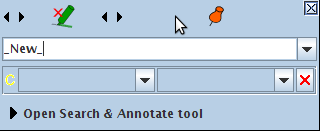
\includegraphics[scale=0.5]{new-annotation.png}
\end{center}
\caption{Creating a New Annotation}
\label{fig:new-annotation}
\end{figure}

The type of the annotation, by default, will be the same as the last annotation
you created, unless there is none, in which case it will be `\_New\_'. You can
enter any annotation type name you wish in the text box, unless you are using
schema-driven annotation (see
Section~\ref{sec:developer:schemaannotationeditor}). You can add or change
features and their values in the table below.

To delete an annotation, click on the red X icon at the top of the popup window.
To grow/shrink the span of the annotation at its start use the two arrow icons on
the left or right and left keys. Use the two arrow icons next on the right to
change the annotation end or alt+right and alt+left keys. Add shift and
control+shift keys to make the span increment bigger. The red X icon is for
removing the annotation.

The pin icon is to pin the window so that it remains where it is. If you drag
and drop the window, this automatically pins it too. Pinning it means that even
if you select another annotation (by hovering over it in the main resource
viewer) it will still stay in the same position.

The popup menu only contains annotation types present in the Annotation Schema
and those already listed in the relevant Annotation Set. To create a new
Annotation Schema, see Section \ref{sec:developer:schemaannotationeditor}. The
popup menu can be edited to add a new annotation type, however.

The new annotation created will automatically be placed in the annotation set
that has been selected (highlighted) by the user. To create a new annotation
set, type the name of the new set to be created in the box below the list of
annotation sets, and click on `New'.

Figure \ref{fig:addAnOrganization} demonstrates adding a `Organization'
annotation for the string `EPSRC' (highlighted in green) to the default
annotation set (blank name in the annotation set view on the right) and a
feature name `type' with a value about to be added.

\begin{figure}[htb]
\begin{center}
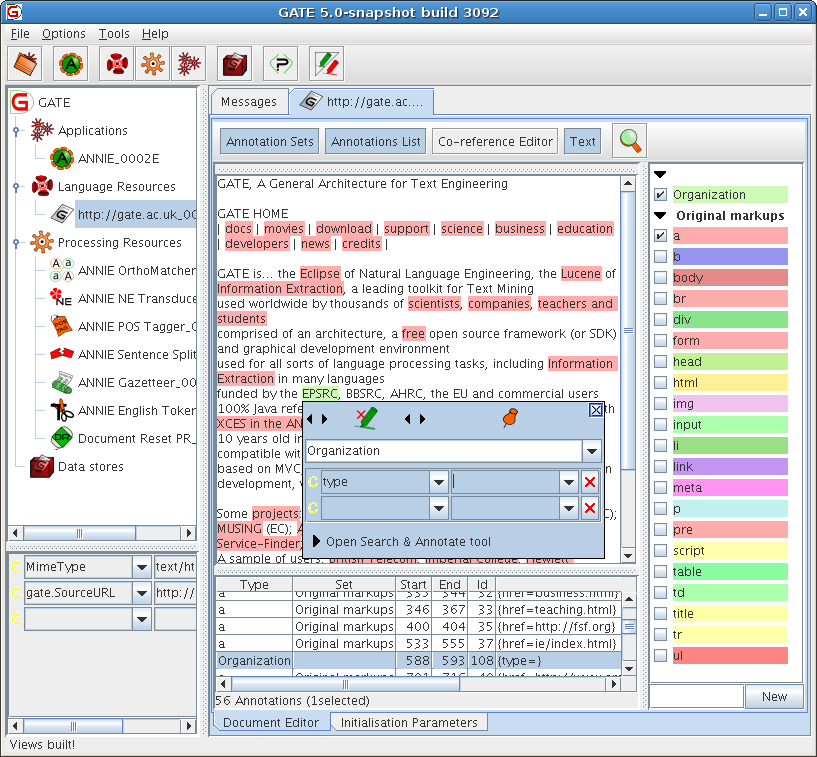
\includegraphics[scale=0.5]{mainWindow.png}
\end{center}
\caption{Adding an Organization annotation to the Default Annotation
Set} \label{fig:addAnOrganization}
\end{figure}

To add a second annotation to a selected piece of text, or to add an overlapping
annotation to an existing one, press the CTRL key to avoid the existing
annotation popup appearing, and then select the text and create the new
annotation. Again by default the last annotation type to have been used will be
displayed; change this to the new annotation type. When a piece of text has more
than one annotation associated with it, on mouseover all the annotations will be
displayed. Selecting one of them will bring up the relevant annotation popup.

\begin{figure}[htb]
\begin{center}
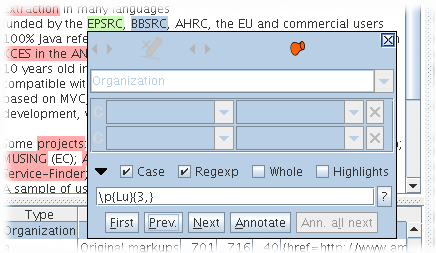
\includegraphics[scale=0.5]{annotation-editor-replace.png}
\end{center}
\caption{Search and Annotate Function of the Annotation Editor.}
\label{fig:searchAnnotateAnnotationEditor}
\end{figure}

To search and annotate the document automatically, use the search and
annotate function as shown in figure
\ref{fig:searchAnnotateAnnotationEditor}:

\begin{itemize}
\item Create and/or select an annotation to be used as a model to annotate.

\item Open the panel at the bottom of the annotation editor window.

\item Change the expression to search if necessary.

\item Use the [First] button or Enter key to select the first expression to
annotate.

\item Use the [Annotate] button if the selection is correct otherwise the
[Next] button. After a few cycles of [Annotate] and [Next], Use the [Ann. all
next] button.
\end{itemize}

Note that after using the [First] button you can move the caret in the
document and use the [Next] button to avoid continuing the search from the
beginning of the document. The [?] button at the end of the search text
field will help you to build powerful regular expressions to search.

%You should next read the section \ref{sec:howto:savingannotations} to save
%annotations.

%%%%%%%%%%%%%%%%%%%%%%%%%%%%%%%%%%%%%%%%%%%%%%%%%%%%%%%%%%%%%%%%%%%%%%%%%%%%%
\subsect[sec:developer:schemaannotationeditor]{Schema-Driven Editing}
%%%%%%%%%%%%%%%%%%%%%%%%%%%%%%%%%%%%%%%%%%%%%%%%%%%%%%%%%%%%%%%%%%%%%%%%%%%%%

Annotation schemas allow annotation types and features to be pre-specified, so
that during manual annotation, the relevant options appear on the drop-down lists
in the annotation editor. You can see some example annotation schemas in
Section~\ref{sec:corpora:schemas}. Annotation schemas provide a means to define
types of annotations in GATE Developer. Basically this means that GATE Developer
`knows about' annotations defined in a schema.
Annotation schemas are supported by the `Annotation schema' language resource,
which is one of the default LR types (along with corpus and document) available
in GATE without the need to load any plugins.

To load an annotation schema into GATE Developer, right-click on `Language
Resources' in the resources pane. Select `New' then `Annotation schema'. A
popup box will appear in which you can browse to your annotation schema XML
file.  A default set of annotation schemas for common annotation types
including Person, Organization and Location is provided in the ANNIE plugin,
and can be loaded by creating an Annotation schema LR from the file {\tt
plugins/ANNIE/resources/schema/ANNIE-Schemas.xml} in the GATE distribution.
You can also define your own schemas to tell GATE Developer about other kinds
of annotations you frequently use.  Each schema file can define only one
annotation type, but you can have a master file which includes others, in order
to load a group of schemas in one operation.  The ANNIE schemas provide an
example of this technique.

By default GATE Developer will allow you to create any annotations in a
document, whether or not there is a schema to describe them.  An alternative
annotation editor component is available which constrains the available
annotation types and features much more tightly, based on the annotation
schemas that are currently loaded.  This is particularly useful when annotating
large quantities of data or for use by less skilled users.

To use this, you must load the \verb|Schema_Annotation_Editor| plugin. With
this plugin loaded, the annotation editor will \emph{only} offer the annotation
types permitted by the currently loaded set of schemas, and when you select an
annotation type only the features permitted by the schema are available to
edit\footnote{Existing features take precedence over the schema, e.g. those created by
previously-run processing resources, are not editable but are not modified or
removed by the editor.}.  Where a feature is declared as having an enumerated
type the available enumeration values are presented as an array of buttons,
making it easy to select the required value quickly.

%%%%%%%%%%%%%%%%%%%%%%%%%%%%%%%%%%%%%%%%%%%%%%%%%%%%%%%%%%%%%%%%%%%%%%%%%%%%%
\subsect[sec:developer:printing]{Printing Text with Annotations}
%%%%%%%%%%%%%%%%%%%%%%%%%%%%%%%%%%%%%%%%%%%%%%%%%%%%%%%%%%%%%%%%%%%%%%%%%%%%%

We suggest you to use your browser to print a document as GATE don't
propose a printing facility for the moment.

First save your document by right clicking on the document in the left
resources tree then choose `Save Preserving Format'. You will get an XML
file with all the annotations highlighted as XML tags plus the `Original
markups' annotations set.

It's possible that the output will not have an XML header and footer because
the document was created from a plain text document. In that case you can
use the XHTML example below.

Then add a stylesheet processing instruction at the beginning of the XML
file, the second line in the following minimalist XHTML document:

\begin{small}\begin{verbatim}
<?xml version="1.0" encoding="UTF-8" ?>
<?xml-stylesheet type="text/css" href="gate.css"?>
<!DOCTYPE html
     PUBLIC "-//W3C//DTD XHTML 1.0 Strict//EN"
    "http://www.w3.org/TR/xhtml1/DTD/xhtml1-strict.dtd">
<html xmlns="http://www.w3.org/1999/xhtml" xml:lang="en" lang="en">
  <head>
    <title>Virtual Library</title>
  </head>
  <body>
  <p>Content of the document</p>
  ...
  </body>
</html>
\end{verbatim}\end{small}

And create a file `gate.css' in the same directory:
\begin{small}\begin{verbatim}
BODY, body { margin: 2em } /* or any other first level tag */
P, p { display: block } /* or any other paragraph tag */
/* ANNIE tags but you can use whatever tags you want */
/* be careful that XML tags are case sensitive */
Date         { background-color: rgb(230, 150, 150) }
FirstPerson  { background-color: rgb(150, 230, 150) }
Identifier   { background-color: rgb(150, 150, 230) }
JobTitle     { background-color: rgb(150, 230, 230) }
Location     { background-color: rgb(230, 150, 230) }
Money        { background-color: rgb(230, 230, 150) }
Organization { background-color: rgb(230, 200, 200) }
Percent      { background-color: rgb(200, 230, 200) }
Person       { background-color: rgb(200, 200, 230) }
Title        { background-color: rgb(200, 230, 230) }
Unknown      { background-color: rgb(230, 200, 230) }
Etc          { background-color: rgb(230, 230, 200) }
/* The next block is an example for having a small tag
   with the name of the annotation type after each annotation */
Date:after {
content: "Date";
font-size: 50%;
vertical-align: sub;
color: rgb(100, 100, 100);
}
\end{verbatim}\end{small}

Finally open the XML file in your browser and print it.

Note that overlapping annotations, cannot be expressed correctly with inline
XML tags and thus won't be displayed correctly.

%%%%%%%%%%%%%%%%%%%%%%%%%%%%%%%%%%%%%%%%%%%%%%%%%%%%%%%%%%%%%%%%%%%%%%%%%%%%%
\sect[sec:developer:plugins]{Using CREOLE Plugins}
%%%%%%%%%%%%%%%%%%%%%%%%%%%%%%%%%%%%%%%%%%%%%%%%%%%%%%%%%%%%%%%%%%%%%%%%%%%%%

In GATE, processing resources are used to automatically create and manipulate
annotations on documents. We will talk about processing resources in the next
section. However, we must first introduce CREOLE plugins. In most cases, in order
to use a particular processing resource (and certain language resources) you must
first load the CREOLE plugin that contains it. This section talks about using
CREOLE plugins. Then, in Section~\ref{sec:developer:loadpr}, we will talk about
creating and using processing resources.

The definitions of CREOLE resources (e.g. processing resources such as taggers
and parsers, see \Chapthing\ \ref{chap:creole-model}) are stored in Maven central repository.


%CREOLE
%directories (directories containing an XML file describing the resources, the
%Java archive with the compiled executable code and whatever libraries are
%required by the resources).

Plugins can have one or more of the following states in relation with GATE:
\begin{description}
\item[known] plugins are those plugins that the system knows about. These
include all the plugins: 1. default plugins provided by Gate team. 2. The plugins 
added by the user manually according to the Maven artifact id. 3. those installed in 
the user's own plugin directory.
\item[loaded] plugins are the plugins currently loaded in the system. All CREOLE
resource types from the loaded plugins are available for use. All known plugins
can easily be loaded and unloaded using the user interface.
\item[auto-loadable] plugins are the list of plugins that the system loads
automatically during initialisation which can be configured via the
{\tt load.plugin.path} system property.
\end{description}

As hinted at above plugnis can be loaded from numerous sources:
\begin{description}
%\item[core plugins] are distributed with GATE are found in the {\\t plugins}
%directory of the instillation, although the default location can be modified using the
%{\tt gate.plugins.home} system property.
\item[core plugins] are distributed with GATE to the Maven central repository.
\item[maven plugins] are distributed with other parties to the Maven central repository.
\item[user plugins] are plugins that have been installed by the user into their
personal plugins folder. The location of this folder can be set either through the
configuration tab of the CREOLE manager interface or via the {\tt gate.user.plugins}
system property
\item[remote plugins] are plugins which are loaded via http from a remote machine.
\end{description}

The CREOLE plugins can be managed through the graphical user interface which can
be activated by selecting `Manage CREOLE Plugins' from the `File' menu. This
will bring up a window listing all the known plugins. For each plugin there are
two check-boxes -- one labelled `Load Now', which will load the plugin, and the
other labelled `Load Always' which will add the plugin to the list of
auto-loadable plugins. A `Delete' button is also provided -- which will remove
the plugin from the list of known plugins. This operation does not delete the 
actual plugin directory. Installed plugins are found automatically when GATE is
started; if an installed plugin is deleted from the list, it will re-appear next 
time GATE is launched.

\begin{figure}[htb]
\begin{center}
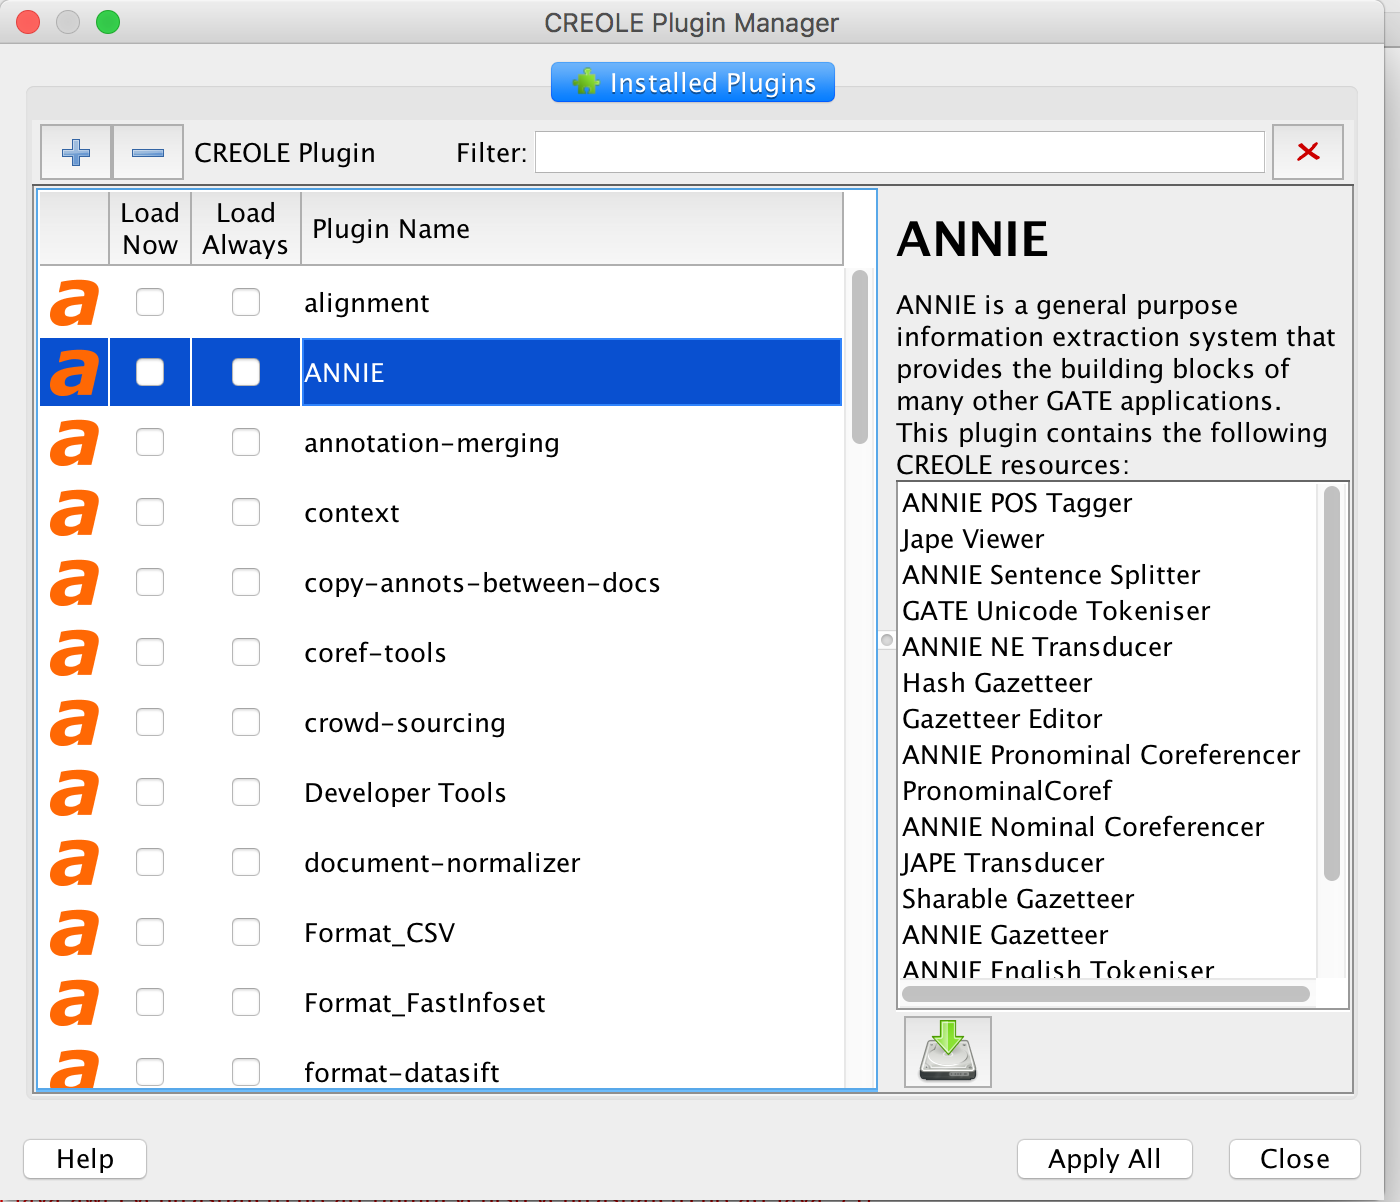
\includegraphics[width=14cm]{creole-manager85.png}
\end{center}
\caption{Plugin Management Console}
\label{fig:plugin-manager}
\end{figure}

If you select a plugin, you will see in the pane on the right the list of
resources that plugin contains. For example, in figure~\ref{fig:plugin-manager},
the `ANNIE' plugin is selected, and you can see that it contains 17 resources.
If you wish to use a
particular resource you will have to ascertain which plugin contains it. This
list can be useful for that. Alternatively, the GATE website provides a directory
of \htlink{http://gate.ac.uk/gate/doc/plugins.html}{plugins and their
processing resources}.

Having loaded the plugins you need, the resources they define will be available
for use. Typically, to the GATE Developer user, this means that they will appear
on the `New' menu when you right-click on `Processing Resources' in the resources
pane, although some special plugins have different effects; for example, the
Schema\_Annotation\_Editor (see
Section~\ref{sec:developer:schemaannotationeditor}).



Extract Plugin Resources  --- ?



%%%%%%%%%%%%%%%%%%%%%%%%%%%%%%%%%%%%%%%%%%%%%%%%%%%%%%%%%%%%%%%%%%%%%%%%%%%%%
\sect[sec:developer:installplugins]{Installing and updating CREOLE Plugins}
%%%%%%%%%%%%%%%%%%%%%%%%%%%%%%%%%%%%%%%%%%%%%%%%%%%%%%%%%%%%%%%%%%%%%%%%%%%%%

While GATE is distributed with a number of core plugins (see Part \ref{part:plugins})
there are many more plugins developed and made available by other GATE users.
Some of these additional plugins can easily be installed into your local copy of
GATE through the CREOLE plugin manager.

%Plugin developers can offer their plugins by maintaining a plugin repository.
%The addresse of a plugin repository can then be added to your GATE installation
%through the configuration tab of the plugin manager. For example, in the following
%screenshot you can see that two plugin repositories have been added, although
%only one is currently enabled.

\begin{figure}[htb]
\begin{center}
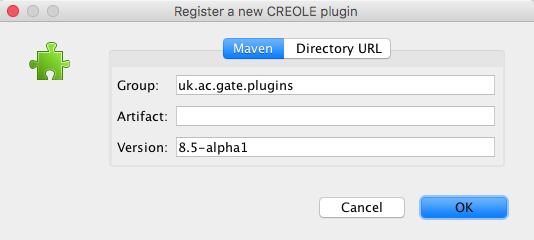
\includegraphics[width=14cm]{registernewplugin.png}
\end{center}
\caption{Installing New CREOLE Plugins Through The Manager}
\label{fig:plugin-manager-config}
\end{figure}

%References to a number of plugin repositories are provided within the GATE distribution,
%although they are initially disabled\footnote{Currently three plugin repositories are listed
%in the main distribution. To have your repository included in the list send an e-mail
%with the address to the GATE developers mailing list.}. Once a plugin repository
%is enabled the plugins which can be installed are listed on the `Available' tab.

Installing new plugins is simply a case of checking the box and clicking `Apply All'.
Note that plugins are installed into the user plugins directory, which must have been
correctly configured before you can try installing new plugins.

Once a plugin is installed it will appear in the list of `Installed Plugins' and can be
loaded in the same way as any other CREOLE plugin (see Section \ref{sec:developer:loadpr}).
If a new version of a plugin you have installed becomes available the new version
will be offered as an update. These updates can be installed in the same way as a new plugin.

To register a new plugin just need simply click the `+' button located at the top right corner of Plugin Manager
Then you can either register a new plugin by provide the Maven Group and Artifact ID for maven plugins or provide the Dirctory URL 
for local or remote plugins.






%%%%%%%%%%%%%%%%%%%%%%%%%%%%%%%%%%%%%%%%%%%%%%%%%%%%%%%%%%%%%%%%%%%%%%%%%%%%%
\sect[sec:developer:loadpr]{Loading and Using Processing Resources}
%%%%%%%%%%%%%%%%%%%%%%%%%%%%%%%%%%%%%%%%%%%%%%%%%%%%%%%%%%%%%%%%%%%%%%%%%%%%%

This section describes how to load and run CREOLE resources not present in ANNIE.
To load ANNIE, see Section \ref{sec:developer:annie}. For technical descriptions
of these resources, see the appropriate chapter in Part~\ref{part:plugins}
(e.g. \Chapthing~\ref{chap:misc-creole}). First ensure that the necessary
plugins have been loaded (see Section \ref{sec:developer:plugins}). If the resource you
require does not appear in the list of Processing Resources, then you probably do
not have the necessary plugin loaded. Processing resources are loaded by
selecting them from the set of Processing Resources: right click on Processing
Resources or select `New Processing Resource' from the File menu.

For example, use the Plugin Console Manager to load the `Tools' plugin. When you
right click on `Processing Resources' in the resources pane and select `New' you
have the option to create any of the processing resources that plugin provides.
You may choose to create a `GATE Morphological Analyser', with the default
parameters. Having done this, an instance of the GATE Morphological Analyser
appears under `Processing Resources'. This processing resource, or PR, is now
available to use. Double-clicking on it in the resources pane reveals its
initialisation parameters, see figure~\ref{fig:pr-init-params}.

\begin{figure}[htb]
\begin{center}
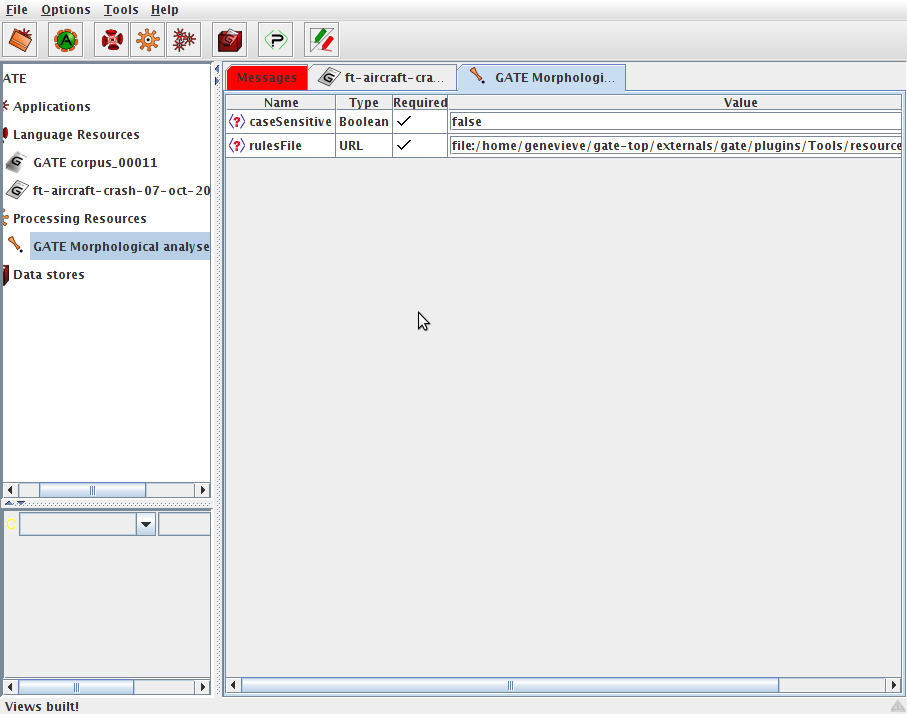
\includegraphics[scale=0.5]{pr-init-params.png}
\end{center}
\caption{GATE Morphological Analyser Initialisation Parameters}
\label{fig:pr-init-params}
\end{figure}

This processing resource is now available to be added to applications. It must
be added to an application before it can be applied to documents. You may
create as many of a particular processing resource as you wish, for example
with different initialisation parameters. Section~\ref{sec:developer:apps}
talks about creating and running applications.

See also the \htlink{http://gate.ac.uk/demos/movies.html\#loadPRs}
{movie for loading processing resources}.

%%%%%%%%%%%%%%%%%%%%%%%%%%%%%%%%%%%%%%%%%%%%%%%%%%%%%%%%%%%%%%%%%%%%%%%%%%%%%
\sect[sec:developer:apps]{Creating and Running an Application}
%%%%%%%%%%%%%%%%%%%%%%%%%%%%%%%%%%%%%%%%%%%%%%%%%%%%%%%%%%%%%%%%%%%%%%%%%%%%%

Once all the resources you need have been loaded, an application can be created
from them, and run on your corpus. Right click on `Applications' and select `New'
and then either `Corpus Pipeline' or `Pipeline'. A pipeline application can only
be run over a single document, while a corpus pipeline can be run over a whole
corpus.

To build the pipeline, double click on it, and select the resources needed
to run the application (you may not necessarily wish to use all those
which have been loaded).

Transfer the necessary components from the set of `loaded components'
displayed on the left hand side of the main window to the set of `selected
components' on the right, by selecting each component and clicking on the
left and right arrows, or by double-clicking on each component.

Ensure that the components selected are listed in the correct order for
processing (starting from the top). If not, select a component and move it
up or down the list using the up/down arrows at the left side of the
pane.

Ensure that any parameters necessary are set for each processing resource
(by clicking on the resource from the list of selected resources and
checking the relevant parameters from the pane below). For example, if you
wish to use annotation sets other than the Default one, these must be
defined for each processing resource.

Note that if a corpus pipeline is used, the corpus needs only to be set
once, using the drop-down menu beside the `corpus' box. If a pipeline is
used, the document must be selected for each processing resource
used.

Finally, click on `Run' to run the application on the document or corpus.

See also the \htlink{http://gate.ac.uk/demos/movies.html\#loadPRs}
{movie for loading and running processing resources}.

For how to use the \emph{conditional} versions of the pipelines see Section
\ref{sec:developer:cond} and for saving/restoring the configuration of an
application see Section \ref{sec:developer:savestate}.

%You should next read the section \ref{sec:howto:annie} to do information
%extraction.

%%%%%%%%%%%%%%%%%%%%%%%%%%%%%%%%%%%%%%%%%%%%%%%%%%%%%%%%%%%%%%%%%%%%%%%%%%%%%
\subsect[sec:developer:appsdatastore]{Running an Application on a Datastore}
%%%%%%%%%%%%%%%%%%%%%%%%%%%%%%%%%%%%%%%%%%%%%%%%%%%%%%%%%%%%%%%%%%%%%%%%%%%%%

To avoid loading all your documents at the same time you can run an
application on a datastore corpus.

To do this you need to load your datastore, see
section~\ref{sec:developer:datastores}, and to load the corpus from the
datastore by double clicking on it in the datastore viewer.

Then, in the application viewer, you need to select this corpus in the drop
down list of corpora.

When you run the application on the corpus datastore, each document will be
loaded, processed, saved then unloaded. So at any time there will be only
one document from the datastore corpus loaded. This prevent memory shortage
but is also a little bit slower than if all your documents were already
loaded.

The processed documents are automatically saved back to the datastore so you
may want to use a copy of the datastore to experiment.

Be very careful that if you have some documents from the datastore corpus
already loaded before running the application then they will not be unloaded
nor saved. To save such document you have to right click on it in the
resources tree view and save it to the datastore.

%%%%%%%%%%%%%%%%%%%%%%%%%%%%%%%%%%%%%%%%%%%%%%%%%%%%%%%%%%%%%%%%%%%%%%%%%%%%%
\subsect[sec:developer:cond]{Running PRs Conditionally on Document Features}
%%%%%%%%%%%%%%%%%%%%%%%%%%%%%%%%%%%%%%%%%%%%%%%%%%%%%%%%%%%%%%%%%%%%%%%%%%%%%

The `Conditional Pipeline' and `Conditional Corpus Pipeline' application
types are conditional versions of the pipelines mentioned in Section
\ref{sec:developer:apps} and allow processing resources to be run or not according
to the value of a feature on the document. In terms of graphical interface, the
only addition brought by the conditional versions of the applications is a box
situated underneath the lists of available and selected resources which allows
the user to choose whether the currently selected processing resource will run
always, never or only on the documents that have a particular value for a named
feature.

If the \emph{Yes} option is selected then the corresponding resource will be
run on all the documents processed by the application as in the case of
non-conditional applications. If the \emph{No} option is selected then the
corresponding resource will never be run; the application will simply ignore
its presence. This option can be used to temporarily and quickly disable an
application component, for debugging purposes for example.

The \emph{If value of feature} option permits running specific application
components conditionally on document features. When selected, this option
enables two text input fields that are used to enter the name of a feature and
the value of that feature for which the corresponding processing resource will
be run. When a conditional application is run over a document, for each
component that has an associated condition, the value of the named feature is
checked on the document and the component will only be used if the value
entered by the user matches the one contained in the document features.

At first sight the conditional behaviour available with these controller may
seem limited, but in fact it is very powerful when used in conjunction with
JAPE grammars (see chapter~\ref{chap:jape}).  Complex conditions can be encoded
in JAPE rules which set the appropriate feature values on the document for use
by the conditional controllers.  Alternatively, the Groovy plugin provides a
\emph{scriptable} controller (see section~\ref{sec:api:groovy:controller}) in
which the execution strategy is defined by a Groovy script, allowing much
richer conditional behaviour to be encoded directly in the controller's
configuration.

%%%%%%%%%%%%%%%%%%%%%%%%%%%%%%%%%%%%%%%%%%%%%%%%%%%%%%%%%%%%%%%%%%%%%%%%%%%%%
\subsect[sec:developer:annie]{Doing Information Extraction with ANNIE}
%%%%%%%%%%%%%%%%%%%%%%%%%%%%%%%%%%%%%%%%%%%%%%%%%%%%%%%%%%%%%%%%%%%%%%%%%%%%%

This section describes how to load and run ANNIE (see
\Chapthing~\ref{chap:annie}) from GATE Developer. ANNIE is a good place to
start because it provides a complete information extraction application, that
you can run on any corpus. You can then view the effects.
% To embed ANNIE in
%other software, see Section \ref{sec:api:embed}.

From the File menu, select `Load ANNIE System'. To run it in its
default state, choose `with Defaults'. This will automatically load
all the ANNIE resources, and create a corpus pipeline called ANNIE with the
correct resources selected in the right order, and the default input and
output annotation sets.

If `without Defaults' is selected, the same processing resources
will be loaded, but a popup window will appear for each resource,
which enables the user to specify a name, location and other parameters
for the resource. This is exactly the same procedure as for loading a
processing resource individually, the difference being that the
system automatically selects those resources contained within
ANNIE. When the resources have been loaded, a corpus pipeline called
ANNIE will be created as before.

The next step is to add a corpus (see Section \ref{sec:developer:loadlr}), and
select this corpus from the drop-down corpus menu in the Serial Application
editor. Finally click on `Run' from the Serial Application editor, or by right
clicking on the application name in the resources pane and selecting `Run'.
(Many people prefer to switch to the messages tab, then run their application
by right-clicking on it in the resources pane, because then it is possible to
monitor any messages that appear whilst the application is running.)

To view the results, double click on one of the document contained in the
corpus processed in the left hand tree view. No annotation sets nor
annotations will be shown until annotations are selected in
the annotation sets; the `Default' set is indicated only with an unlabelled
right-arrowhead which must be selected in order to make visible the available
annotations. Open the default annotation set and select some of the annotations
to see what the ANNIE application has done.

See also the \htlink{http://gate.ac.uk/demos/movies.html\#annie}
{movie for loading and running ANNIE}.

%%%%%%%%%%%%%%%%%%%%%%%%%%%%%%%%%%%%%%%%%%%%%%%%%%%%%%%%%%%%%%%%%%%%%%%%%%%%%
\subsect[sec:developer:modifyannie]{Modifying ANNIE}
%%%%%%%%%%%%%%%%%%%%%%%%%%%%%%%%%%%%%%%%%%%%%%%%%%%%%%%%%%%%%%%%%%%%%%%%%%%%%

You will find the ANNIE resources in gate/plugins/ANNIE/resources. Simply locate
the existing resources you want to modify, make a copy with a new name, edit
them, and load the new resources into GATE as new Processing Resources (see
Section \ref{sec:developer:loadpr}).

%%%%%%%%%%%%%%%%%%%%%%%%%%%%%%%%%%%%%%%%%%%%%%%%%%%%%%%%%%%%%%%%%%%%%%%%%%%%%
\sect[sec:developer:saving]{Saving Applications and Language Resources}
%%%%%%%%%%%%%%%%%%%%%%%%%%%%%%%%%%%%%%%%%%%%%%%%%%%%%%%%%%%%%%%%%%%%%%%%%%%%%

In this section, we will describe how applications and language resources can
be saved for use outside of GATE and for use with GATE at a later time.
Section~\ref{sec:developer:dump} talks about saving documents to file.
Section~\ref{sec:developer:datastores} outlines how to use datastores.
Section~\ref{sec:developer:savestate} talks about saving application states
(resource parameter states), and Section~\ref{sec:developer:export} talks about 
exporting applications together with referenced files and resources to a ZIP file.

%%%%%%%%%%%%%%%%%%%%%%%%%%%%%%%%%%%%%%%%%%%%%%%%%%%%%%%%%%%%%%%%%%%%%%%%%%%%%
\subsect[sec:developer:dump]{Saving Documents to File}
%%%%%%%%%%%%%%%%%%%%%%%%%%%%%%%%%%%%%%%%%%%%%%%%%%%%%%%%%%%%%%%%%%%%%%%%%%%%%

There are three main ways to save annotated documents:

\begin{enumerate}
\item\label{item:savepreserve}
preserving the original markup, with optional added annotations;
\item\label{item:saveasxml}
in GATE's own XML serialisation format (including all the annotations on the
document);
\item
by writing your own dump algorithm as a processing resource.
\end{enumerate}

This section describes how to use the first two options.

Both types of data export are available in the popup menu triggered by
right-clicking on a document in the resources tree
(see Section \ref{sec:developer:gui}):
type \ref{item:savepreserve}
is called `Save Preserving Format' and type \ref{item:saveasxml}
is called `Save as XML'. In addition, all documents in a corpus
can be saved as individual XML files into a directory by 
right-clicking on the corpus in the resources tree and choosing
the option `Save as XML`.

Selecting the save as XML option leads to a file open dialogue; give the name
of the file you want to create, and the whole document and all its data will
be exported to that file. If you later create a document from that file, the
state will be restored. ({\bf Note:} because GATE's annotation model is
richer than that of XML, and because our XML dump implementation sometimes
cuts corners\footnote{Gorey details: features of annotations and documents
in GATE may be any virtually any Java object; serialising arbitrary binary
data to XML is not simple; instead we serialise them as strings, and
therefore they will be re-loaded as strings.}, the state may not be identical
after restoration. If your
intention is to store the state for later use, use a DataStore instead.)

The `Save Preserving Format' option also leads to a file dialogue; give a name
and the data you require will be dumped into the file. The action can be used for
documents that were created from files using the XML or HTML format. It will save
all the original tags as well as the document annotations that are currently
displayed in the `Annotations List' view. This option is useful for selectively
saving only some annotation types.

The annotations are saved as normal document tags, using the annotation type as
the tag name. If the advanced option `Include annotation features for ``Save
Preserving Format''' (see Section \ref{sec:gettingstarted:gateconfig}) is set
to true, then the annotation features will also be saved as tag attributes.

Using this operation for GATE documents that were not created from an HTML or XML
file results in a plain text file, with in-line tags for the saved annotations.

Note that GATE's model of annotation allows graph structures, which are difficult
to represent in XML (XML is a tree-structured representation format). During the
dump process, annotations that cross each other in ways that cannot be represented
in legal XML will be discarded, and a warning message printed.

%%%%%%%%%%%%%%%%%%%%%%%%%%%%%%%%%%%%%%%%%%%%%%%%%%%%%%%%%%%%%%%%%%%%%%%%%%%%%
\subsect[sec:developer:datastores]{Saving and Restoring LRs in Datastores}
%%%%%%%%%%%%%%%%%%%%%%%%%%%%%%%%%%%%%%%%%%%%%%%%%%%%%%%%%%%%%%%%%%%%%%%%%%%%%

Where corpora are large, the memory available may not be sufficient to have all
documents open simultaneously. The datastore functionality provides the option
to save documents to disk and open them only one at a time for
processing. This means that much larger corpora can be used. A datastore can
also be useful for saving documents in an efficient and lossless way. 

To save a text in a datastore, a new datastore must first be created if one
does not already exist. Create a datastore by right clicking on Datastore in
the left hand pane, and select the option `Create Datastore'. Select the data
store type you wish to use. Create a directory to be used as the datastore (note
that the datastore is a directory and not a file).

You can either save a whole corpus to the datastore (in which case the structure
of the corpus will be preserved) or you can save individual documents. The
recommended method is to save the whole corpus. To save a corpus, right click on
the corpus name and select  the `Save to...' option (giving the name of the
datastore created earlier). To save individual documents to the datastore, 
right clicking on each document name and follow the same procedure.

To load a document from a datastore, do not try to load it as a language
resource. Instead, open the datastore by right clicking on Datastore in the
left hand pane, select `Open Datastore' and choose the datastore to open.
The datastore tree will appear in the main window. Double click on a corpus or
document in this tree to open it. To save a corpus and document back to the same
datastore, simply select the `Save' option.

See also the \htlink{http://gate.ac.uk/demos/movies.html\#createDataStore}
{movie for creating a datastore} and the
\htlink{http://gate.ac.uk/demos/movies.html\#loadDataStore}
{movie for loading corpus and documents from a datastore}.


%%%%%%%%%%%%%%%%%%%%%%%%%%%%%%%%%%%%%%%%%%%%%%%%%%%%%%%%%%%%%%%%%%%%%%%%%%%%%
\subsect[sec:developer:savestate]{Saving Application States to a File}
%%%%%%%%%%%%%%%%%%%%%%%%%%%%%%%%%%%%%%%%%%%%%%%%%%%%%%%%%%%%%%%%%%%%%%%%%%%%%

Resources, and applications that are made up of them,
are created based on the settings of their parameters (see Section
\ref{sec:developer:loadpr}). It is possible to save the data used to create
an application to a file and re-load it later. To save the
application to a file, right click on it in the resources tree and select
`Save application state', which will give you a file creation dialogue.
Choose a file name that ends in \texttt{gapp} as this file dialog and
the one for loading application states age displays all files which
have a name ending in \texttt{gapp}. A common convention is to 
use \texttt{.gapp} as a file extension.

To restore the application later, select `Restore application from file'
from the `File' menu.

Note that the data that is saved represents how to {\it recreate} an
application -- not the resources that make up the application itself. So,
for example, if your application has a resource that initialises itself from
some file (e.g. a grammar, a document) then that file must still exist when
you restore the application.

In case you don't want to save the corpus configuration associated with the
application then you must select `$<$none$>$' in the corpus list of the
application before saving the application.

The file resulting from saving the application state contains the values of the
initialisation and runtime parameters for all the processing resources contained by the
stored application as well as the values of the initialisation parameters for 
all the language resources referenced by those processing resources. Note that
if you reference a document that has been created with an empty URL and empty
string content parameter and subsequently been manually edited to add content,
that content will not be saved. In order for document content to be preserved,
load the document from an URL, specify the content as for the string content
parameter or use a document from a datastore.

For the parameters of type URL (which are typically used to
select external resources such as grammars or rules files) a transformation is
applied so that  
the paths are are stored relative to either the location of the saved application 
state file, the GATE home directory, or a special user resources home directory,
according to the following rules:
\begin{itemize}
\item If the resource is inside the GATE home directory, but the the application
  state file is saved to a location outside the GATE home directory, the path
  is stored relative to the GATE home directory and the path marker 
  \verb=$gatehome$=
  is used.
\item If the property \texttt{gate.user.resourceshome} is set to the path of
  a directory and the resource
  is located inside that directory but the state file is saved to a location 
  outside of this directory, the path is stored relative to this directory
  and the path marker \verb=$resourceshome$= is used.
\item in all other situations, the path is stored relative to the location of
  the application state file location and the the path marker \verb=$relpath$=
  is used.
\end{itemize}

In this way, all resource files that are part of GATE are always used corretly,
no matter where GATE is installed. Resource files which are not part of GATE
and used by an application do not need to be in the same location as when the 
application was initially created but rather in the same \emph{location relative 
to the location of the application file}. 
In addition if your application uses a project-specific location for global
resources or project specific plugins, the java property \texttt{gate.user.resourceshome}
can be set to this location and the application will be stored so that this
location will also always be used correctly, no matter where the application state
file is copied to. To set the resources home directory, the \texttt{-rh location} 
option for the Linux script \texttt{gate.sh} to start GATE can be used.
The combination of these features allows the creation and deployment of portable
applications by keeping the application file and the resource files used by the
application together.


Note that GATE resources that are used by your application may change
between different releases of GATE. If your application depends on a specific 
version of resources that come with the GATE distribution, consider copying them
to your project directory in order to ensure the correct version is used.
The option "Export for GATE Cloud" (see
Section~\ref{sec:developer:export})
 supports this by creating a ZIP file that
contains a copy all GATE resources used by the application, including GATE plugins.

When an application is restored from an application state file, 
GATE uses the keyword \verb=$relpath$= for paths relative to the location of the
gapp file, \verb=$gatehome$= for paths relative to the GATE home installation directory
and \verb=$resourceshom$= for paths relative to the the location the property
\texttt{gate.user.resourceshome} is set. 
There exists other keywords that can be interesting in some
cases. You will need to edit the gapp file manually. The keywords are
\verb=$gateplugins$= and \verb=$sysprop:...$=. The latter is any java
system property, for example \verb=$sysprop:user.home$=.

If you want to save your application along with all the resources it requires
you can use the `Export for GATE Cloud' option (see
Section~\ref{sec:developer:export}).

See also the \htlink{http://gate.ac.uk/demos/movies.html\#saveAppState}
{movie for saving and restoring applications}.

%%%%%%%%%%%%%%%%%%%%%%%%%%%%%%%%%%%%%%%%%%%%%%%%%%%%%%%%%%%%%%%%%%%%%%%%%%%%%
\subsect[sec:developer:export]{Saving an Application with its Resources
(e.g. GATE Cloud)}
%%%%%%%%%%%%%%%%%%%%%%%%%%%%%%%%%%%%%%%%%%%%%%%%%%%%%%%%%%%%%%%%%%%%%%%%%%%%%

When you save an application using the `Save application state' option
(see Section~\ref{sec:developer:savestate}), the saved file contains references
to the plugins that were loaded when the application was saved, and to any
resource files required by the application.  To be able to reload the file,
these plugins and other dependencies must exist at the same locations
(relative to the saved state file).  While this is fine for saving and
loading applications on a single machine it means that if you want to
package your application to run it elsewhere (e.g. deploy it to 
\htlink{https://cloud.gate.ac.uk}{GATE Cloud}) then
you need to be careful to include all the resource files and plugins at the
right locations in your package.  The `Export for GATE Cloud' option on the
right-click menu for an application helps to automate this process.

When you export an application in this way, GATE Developer produces a
ZIP file containing the saved application state (in the same format as
`Save application state').  Any plugins and resource files that the
application refers to are also included in the zip file, and the
relative paths in the saved state are rewritten to point to the
correct locations within the package.  The resulting package is
therefore self-contained and can be copied to another machine and
unpacked there, or passed to
\htlink{https://cloud.gate.ac.uk}{GATE Cloud} for deployment.

As well as selecting the location where you want to save the package,
the `Export for GATE Cloud' option will also prompt you to select the
annotation sets that your application uses for input and output.  For
example, if your application makes use of the unpacked XML markup in
source documents and creates annotations in the default set then you
would select `Original markups' as an input set and the `{\it
$<$Default annotation set$>$}' as an output set.  GATE Developer will
try to make an educated guess at the correct sets but you should check
and amend the lists as necessary.

There are a few important points to note about the export process:
\begin{itemize}
\item The complete contents of all the plugin directories that are loaded when
  you perform the export will be included in the resulting package.  Use the
  plugin manager to unload any plugins your application is not using before you
  export it.
\item If your application refers to a resource file in a directory that is not
  under one of the loaded plugins, the entire contents of this directory will be
  recursively included in the package.  If you have a number of unrelated
  resources in a single directory (e.g. many sets of large gazetteer lists) you
  may want to separate them into separate directories so that only the relevant
  ones are included in the package.
\item The packager only knows about resources that your application refers to
  directly in its parameters.  For example, if your application includes a
  multi-phase JAPE grammar the packager will only consider the main grammar
  file, not any of its sub-phases.  If the sub-phases are not contained in the
  same directory as the main grammar you may find they are not included.  If
  indirect references of this kind are all to files under the same directory as
  the `master' file it will work OK.
\end{itemize}

If you require more flexibility than this option provides you should read
Section~\ref{sec:ant:packagegapp}, which describes the underlying Ant task that
the exporter uses.

\subsect[sec:developer:convertxgapp]{Upgrade An Application to use Newer Versions of Plugins}
%%%%%%%%%%%%%%%%%%%%%%%%%%%%%%%%%%%%%%%%%%%%%%%%%%%%%%%%%%%%%%%%%%%%%%%%%%%%%
Some of the changes introduced in GATE 8.5 mean that applications saved with a previous version of GATE might not
load without being updated. Loading such an application is likely to result in errors similar to those seen in Figure \ref{fig:oldxgapp}.

\begin{figure}[htb]
\begin{center}
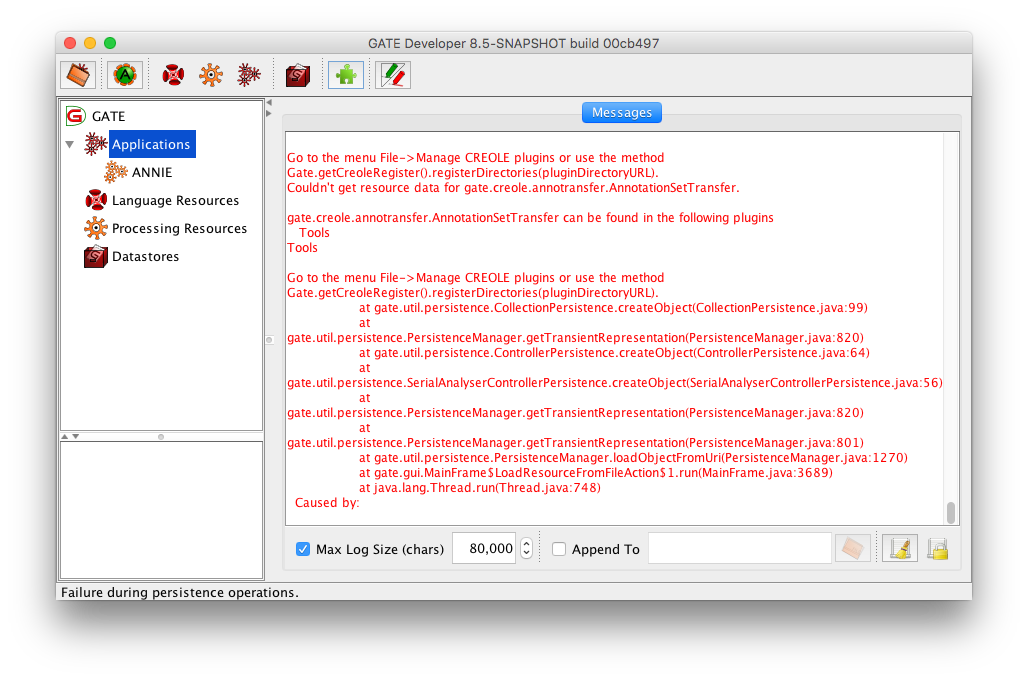
\includegraphics{old-xgapp-error.png}
\end{center}
\caption{Old xgapp version Loading Error}
\label{fig:oldxgapp}
\end{figure}

In order to load such application into GATE 8.5 (or above), you need first upgrade them to use compatible versions of the relevant plugins.
In most cases this process can be automated and we provide a tool to walk you through the process. To start upgrading an application select
`Upgrade XGapp' from the `Tools' menu. This will first ask you to choose an application file to upgrade and will then present the UI shown in
Figure \ref{fig:upgrade-tool}.

\begin{figure}[htb]
\begin{center}
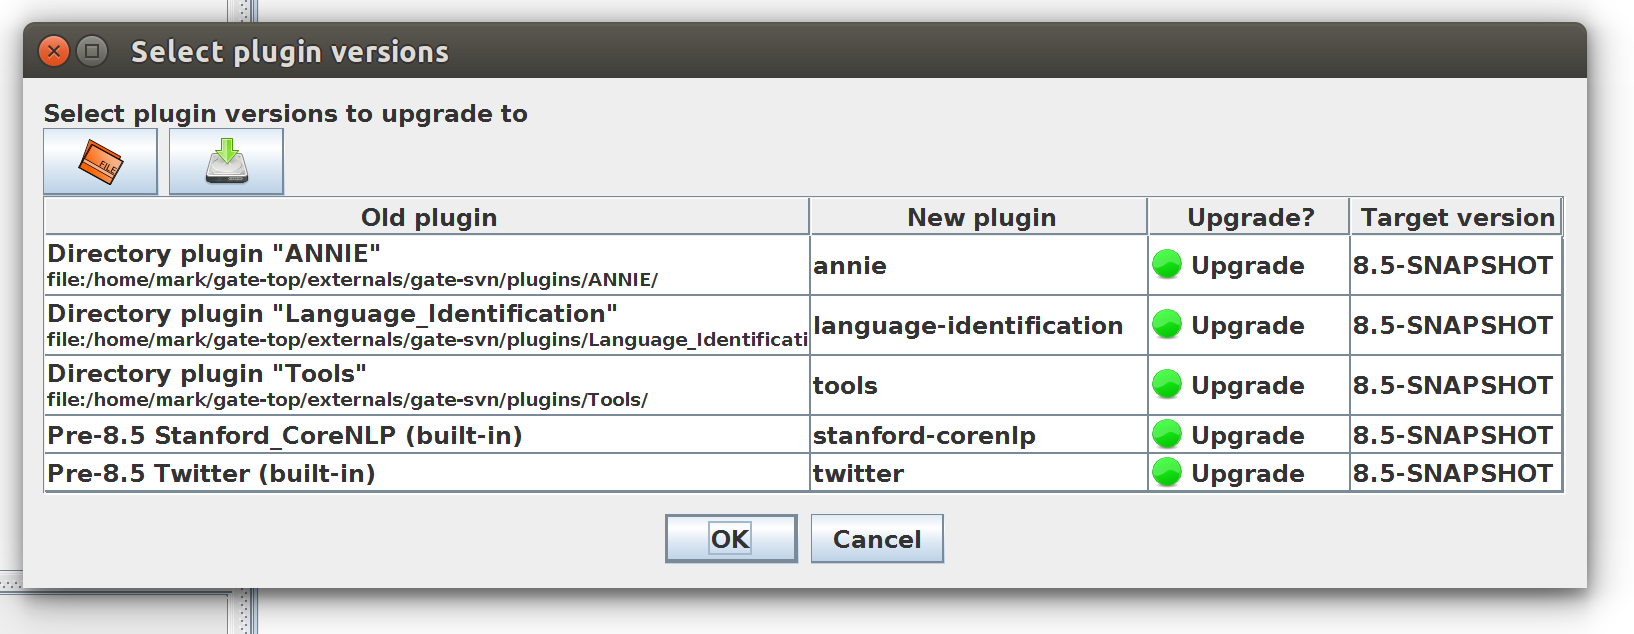
\includegraphics{upgrade-tool.png}
\end{center}
\caption{XGapp Upgrade Tool}
\label{fig:upgrade-tool}
\end{figure}

One the application has been analysed the tool will show you a table in which each row signifies a plugin used by the app. In the left most
column it lists the plugin currently referenced by the application. This is followed by details of the new plugin. While in most cases
the tool can correctly determine the right plugin to offer in this column you can correct any mistakes by double-clicking the incorrect
plugin and then specifying the correct plugin location. The final two columns determine if the plugin is upgraded and to which version.
The versions offered are all those which are available and known to be compatible with the version of GATE you are running. By default the
latest available version will be selected, although -SNAPSHOT versions are only selected by default if you are also running a -SNAPSHOT version
of GATE.

The `Upgrade' column allows you to determine if and how a plugin will be upgraded. The three possible choices are Upgrade, Plugin Only, and Skip.
Skip is fairly self explanatory but upgrade and plugin only require a little more explanation. Upgrade means that not only will the plugin location
be upgraded, but also any resources that reside within the plugin will also be changed to reference those within the new plugin. This is the only
upgrade option when considering a plugin which was originally part of the GATE distribution. The plugin only option allows you to change the application
to load a new version of the plugin which leaving the resource locations untouched. This is useful for cases where you have edited the resources inside a
plugin rather than having created a separate copy specific to the application.

After upgrade, the old version of the application file will still be available but will have been renamed by adding the '.bak' suffix.

In most cases this upgrade process will work without issue. If, however, you find you have an application which fails to open after the upgrade then it
maybe because one or more plugins couldn't be correctly mapped to new versions. In these cases the best option is to revert the upgrade (replace the xgapp file
with the generated backup), load the application into GATE 8.4.1 and then use the ``Export for GATE Cloud'' option to produce a self contained application (see
Section \ref{(see Section~\ref{sec:developer:export})}. Then finally run the upgrade tool over this version of the application.

The two buttons at the top of the dialog allow you save and restore the mappings defined in the table. This makes it easier to upgrade a set of
related applications which should all be upgraded in a similar fashion.

Note that this process is not limited simply to upgrading applications saved prior to GATE 8.5 but can be used at any time to upgrade
the version of a plugin used by an application.

%%%%%%%%%%%%%%%%%%%%%%%%%%%%%%%%%%%%%%%%%%%%%%%%%%%%%%%%%%%%%%%%%%%%%%%%%%%%%
\sect[sec:developer:keyboard]{Keyboard Shortcuts}
%%%%%%%%%%%%%%%%%%%%%%%%%%%%%%%%%%%%%%%%%%%%%%%%%%%%%%%%%%%%%%%%%%%%%%%%%%%%%

You can use various keyboard shortcuts for common tasks in GATE Developer.
These are listed in this section.

{\bf General (Section \ref{sec:developer:gui}):}

\begin{itemize}
\item {\bf F1} Display a help page for the selected component
\item {\bf Alt+F4} Exit the application without confirmation
\item {\bf Tab} Put the focus on the next component or frame
\item {\bf Shift+Tab} Put the focus on the previous component or frame
\item {\bf F6} Put the focus on the next frame
\item {\bf Shift+F6} Put the focus on the previous frame
\item {\bf Alt+F} Show the File menu
\item {\bf Alt+O} Show the Options menu
\item {\bf Alt+T} Show the Tools menu
\item {\bf Alt+H} Show the Help menu
\item {\bf F10} Show the first menu
\end{itemize}


{\bf Resources tree (Section \ref{sec:developer:gui}):}

\begin{itemize}
\item {\bf Enter} Show the selected resources
\item {\bf Ctrl+H} Hide the selected resource
\item {\bf Ctrl+Shift+H} Hide all the resources
\item {\bf F2} Rename the selected resource
\item {\bf Ctrl+F4} Close the selected resource
\end{itemize}

{\bf Document editor (Section \ref{sec:developer:documents}):}

\begin{itemize}
\item {\bf Ctrl+F} Show the search dialog for the document
\item {\bf Ctrl+E} Edit the annotation at the caret position
\item {\bf Ctrl+S} Save the document in a file
\item {\bf F3} Show/Hide the annotation sets
\item {\bf Shift+F3} Show the annotation sets with preselection
\item {\bf F4} Show/Hide the annotations list
\item {\bf F5} Show/Hide the coreference editor
\item {\bf F7} Show/Hide the text
\end{itemize}

{\bf Annotation editor (Section \ref{sec:developer:annotations}):}

\begin{itemize}
\item {\bf Right/Left} Grow/Shrink the annotation span at its start
\item {\bf Alt+Right/Alt+Left} Grow/Shrink the annotation span at its end
\item {\bf +Shift/+Ctrl+Shift} Use a span increment of 5/10 characters
\item {\bf Alt+Delete} Delete the currently edited annotation
\end{itemize}

{\bf Annic/Lucene datastore (\Chapthing~\ref{chap:annic}):}

\begin{itemize}
\item {\bf Alt+Enter} Search the expression in the datastore
\item {\bf Alt+Backspace} Delete the search expression
\item {\bf Alt+Right} Display the next page of results
\item {\bf Alt+Left} Display the row manager
\item {\bf Alt+E} Export the results to a file
\end{itemize}

{\bf Annic/Lucene query text field (\Chapthing~\ref{chap:annic}):}

\begin{itemize}
\item {\bf Ctrl+Enter} Insert a new line
\item {\bf Enter} Search the expression
\item {\bf Alt+Top} Select the previous result
\item {\bf Alt+Bottom} Select the next result
\end{itemize}


%%%%%%%%%%%%%%%%%%%%%%%%%%%%%%%%%%%%%%%%%%%%%%%%%%%%%%%%%%%%%%%%%%%%%%%%%%%%%
\sect[sec:developer:misc]{Miscellaneous}
%%%%%%%%%%%%%%%%%%%%%%%%%%%%%%%%%%%%%%%%%%%%%%%%%%%%%%%%%%%%%%%%%%%%%%%%%%%%%

%%%%%%%%%%%%%%%%%%%%%%%%%%%%%%%%%%%%%%%%%%%%%%%%%%%%%%%%%%%%%%%%%%%%%%%%%%%%%
\subsect[sec:developer:deletesession]{Stopping GATE from Restoring Developer
Sessions/Options}
%%%%%%%%%%%%%%%%%%%%%%%%%%%%%%%%%%%%%%%%%%%%%%%%%%%%%%%%%%%%%%%%%%%%%%%%%%%%%

GATE can remember Developer options and the state of the resource tree when it
exits. The options are saved by default; the session state is not saved by
default. This default behaviour can be changed from the `Advanced' tab of
the `Configuration' choice on the `Options' menu.

If a problem occurs and the saved data prevents GATE Developer from
starting, you can fix this by deleting the configuration and session
data files. These are stored in your home directory, and are called
{\tt gate.xml} and {\tt gate.sesssion} or {\tt .gate.xml} and {\tt
.gate.sesssion} depending on platform.  On Windows your home is:
\begin{description}
\item[95, 98, NT:] Windows Directory/profiles/username
\item[2000, XP:] Windows Drive/Documents and Settings/username
\end{description}


%%%%%%%%%%%%%%%%%%%%%%%%%%%%%%%%%%%%%%%%%%%%%%%%%%%%%%%%%%%%%%%%%%%%%%%%%%%%%
\subsect[sec:developer:unicode]{Working with Unicode}
%%%%%%%%%%%%%%%%%%%%%%%%%%%%%%%%%%%%%%%%%%%%%%%%%%%%%%%%%%%%%%%%%%%%%%%%%%%%%

When you create a document from a URL pointing to textual data
in GATE, you have to tell the system what character encoding the text is
stored in. By default, GATE will set this parameter to be the empty string.
This tells Java to use the default encoding for whatever platform it is
running on at the time -- e.g. on Western versions of Windows this will be
ISO-8859-1, and Eastern ones ISO-8859-9. On Linux systems, the default 
encoding is influenced by the \texttt{LANG} environment variable, e.g.
when this variable is set to \texttt{en\_US.utf-8} the default encoding used
will be \texttt{UTF-8}. When GATE is started using the \texttt{bin/ant run} 
command or (on Linux) through the \texttt{gate.sh} script or a link to it,
you can change the default encoding used by GATE to UTF-8 by adding 
\texttt{-Drun.file.encoding=utf-8} as a parameter.

A popular way to store Unicode
documents is in UTF-8, which is a superset of ASCII (but can still store all
Unicode data); if you get
an error message about document I/O during reading, try setting the encoding
to UTF-8, or some other locally popular encoding.

%%%%%%%%%%%%%%%%%%%%%%%%%%%%%%%%%%%%%%%%%%%%%%%%%%%%%%%%%%%%%%%%%%%%%%%%%%%%%
